%!TEX program = xelatex
%!BIB program = bibtex

\documentclass[en,black,10pt,normal]{elegantnote}
\usepackage{float}
\usepackage{hyperref}
\usepackage{subfigure}
\usepackage{svg}


\newcommand{\upcite}[1]{\textsuperscript{\textsuperscript{\cite{#1}}}}

\title{Practical 5 BLAST II}
\author{WenYuan Jiang\\ID: 1951510}
\institute{School of Life Science, Tongji University}
%\version{1.00}
\date{April 23, 2021}
\lstset{basicstyle=\footnotesize\ttfamily}
\AtBeginEnvironment{lstlisting}{\linespread{0.75}\selectfont}

\begin{document}

\maketitle

\section{In this section, you will learn how to build your own BLAST-searchable database.}

There are two FASTA format files which consists of sequences of corona virus, 
format them to a blast-searchable database respectively. 
Here we have a list  
of accession numbers for query sequences. Please blast the query sequences in the local databases and show your best results.

\begin{itemize}
    \item MT186683
    \item NP\_002200
\end{itemize}

\subsection{Install BLAST}

We downloaded the source code from NCBI and complied
the code on a local linux machine. The commands used is shown below.

\begin{lstlisting}
# wget https://ftp.ncbi.nlm.nih.gov/blast/executables/LATEST/ncbi-blast-2.11.0+-src.tar.gz
# tar -xvf ncbi-blast-2.11.0+-src.tar.gz
# cd ncbi-blast-2.11.0+-src/c++
# ./configure & make -j & make install
\end{lstlisting}



\subsection{Download the databases and the sequences}
We downloaded the fasta files to build our database from the class canvas platform.

(\url{http://canvas.tongji.edu.cn/courses/41137/files/folder/%E4%BD%9C%E4%B8%9A%E4%BA%94})


The files are listed below.
\begin{itemize}
    \item \lstinline{coronavirus.fasta}
    \item \lstinline{SARS2_NCBIVirus_complete_genomes_20200329.fasta}
\end{itemize}

The sequences used in the query is fetched from \texttt{NCBI} using \lstinline{Entrez} system.

The commands used to fetch the query sequences is shown in supplement.

\subsection{Creating BLAST database}

First, we examined the fasta files used in building a blast database.

\begin{lstlisting}
root@2cfa8ee205ce:~/exp5# cat db.fasta | grep '^>' | wc -l \                                             
> # Total sequences number of the database source file
198
root@2cfa8ee205ce:~/exp5# cat db.fasta | grep -v '^>'| grep -o '[ATCG]' | wc -l \ 
> # Total chars
5893214
root@2cfa8ee205ce:~/exp5# ls -hl db.fasta 
-rw-r--r-- 1 1000 1000 5.8M Apr 23 12:50 db.fasta
\end{lstlisting}

Since the file used to create the blast database is not large,
we used default parameters to build the database.
\begin{lstlisting}
root@2cfa8ee205ce:~/exp5# makeblastdb -in db.fasta -out db -dbtype nucl


Building a new DB, current time: 04/23/2021 15:05:20
New DB name:   /root/exp5/db
New DB title:  db.fasta
Sequence type: Nucleotide
Deleted existing Nucleotide BLAST database named /root/exp5/db
Keep MBits: T
Maximum file size: 1000000000B
Adding sequences from FASTA; added 198 sequences in 0.0501249 seconds.
\end{lstlisting}



\subsection{Blasting \texttt{MT186683}}

\subsubsection{Results overview}

\begin{figure}[H]
  \centering
  \subfigure[MN908947]{
\includegraphics[width=1.8in]{B1}}
  \subfigure[BetaCoV\_pangolin\_Guangxi\_P1E]{
\includegraphics[width=1.8in]{B2}}
  \subfigure[MG772934]{
\includegraphics[width=1.8in]{B3}}\\
  \subfigure[DQ412042]{
\includegraphics[width=1.8in]{B4}}
  \subfigure[BetaCoV\_pangolin\_Guangxi\_P3B]{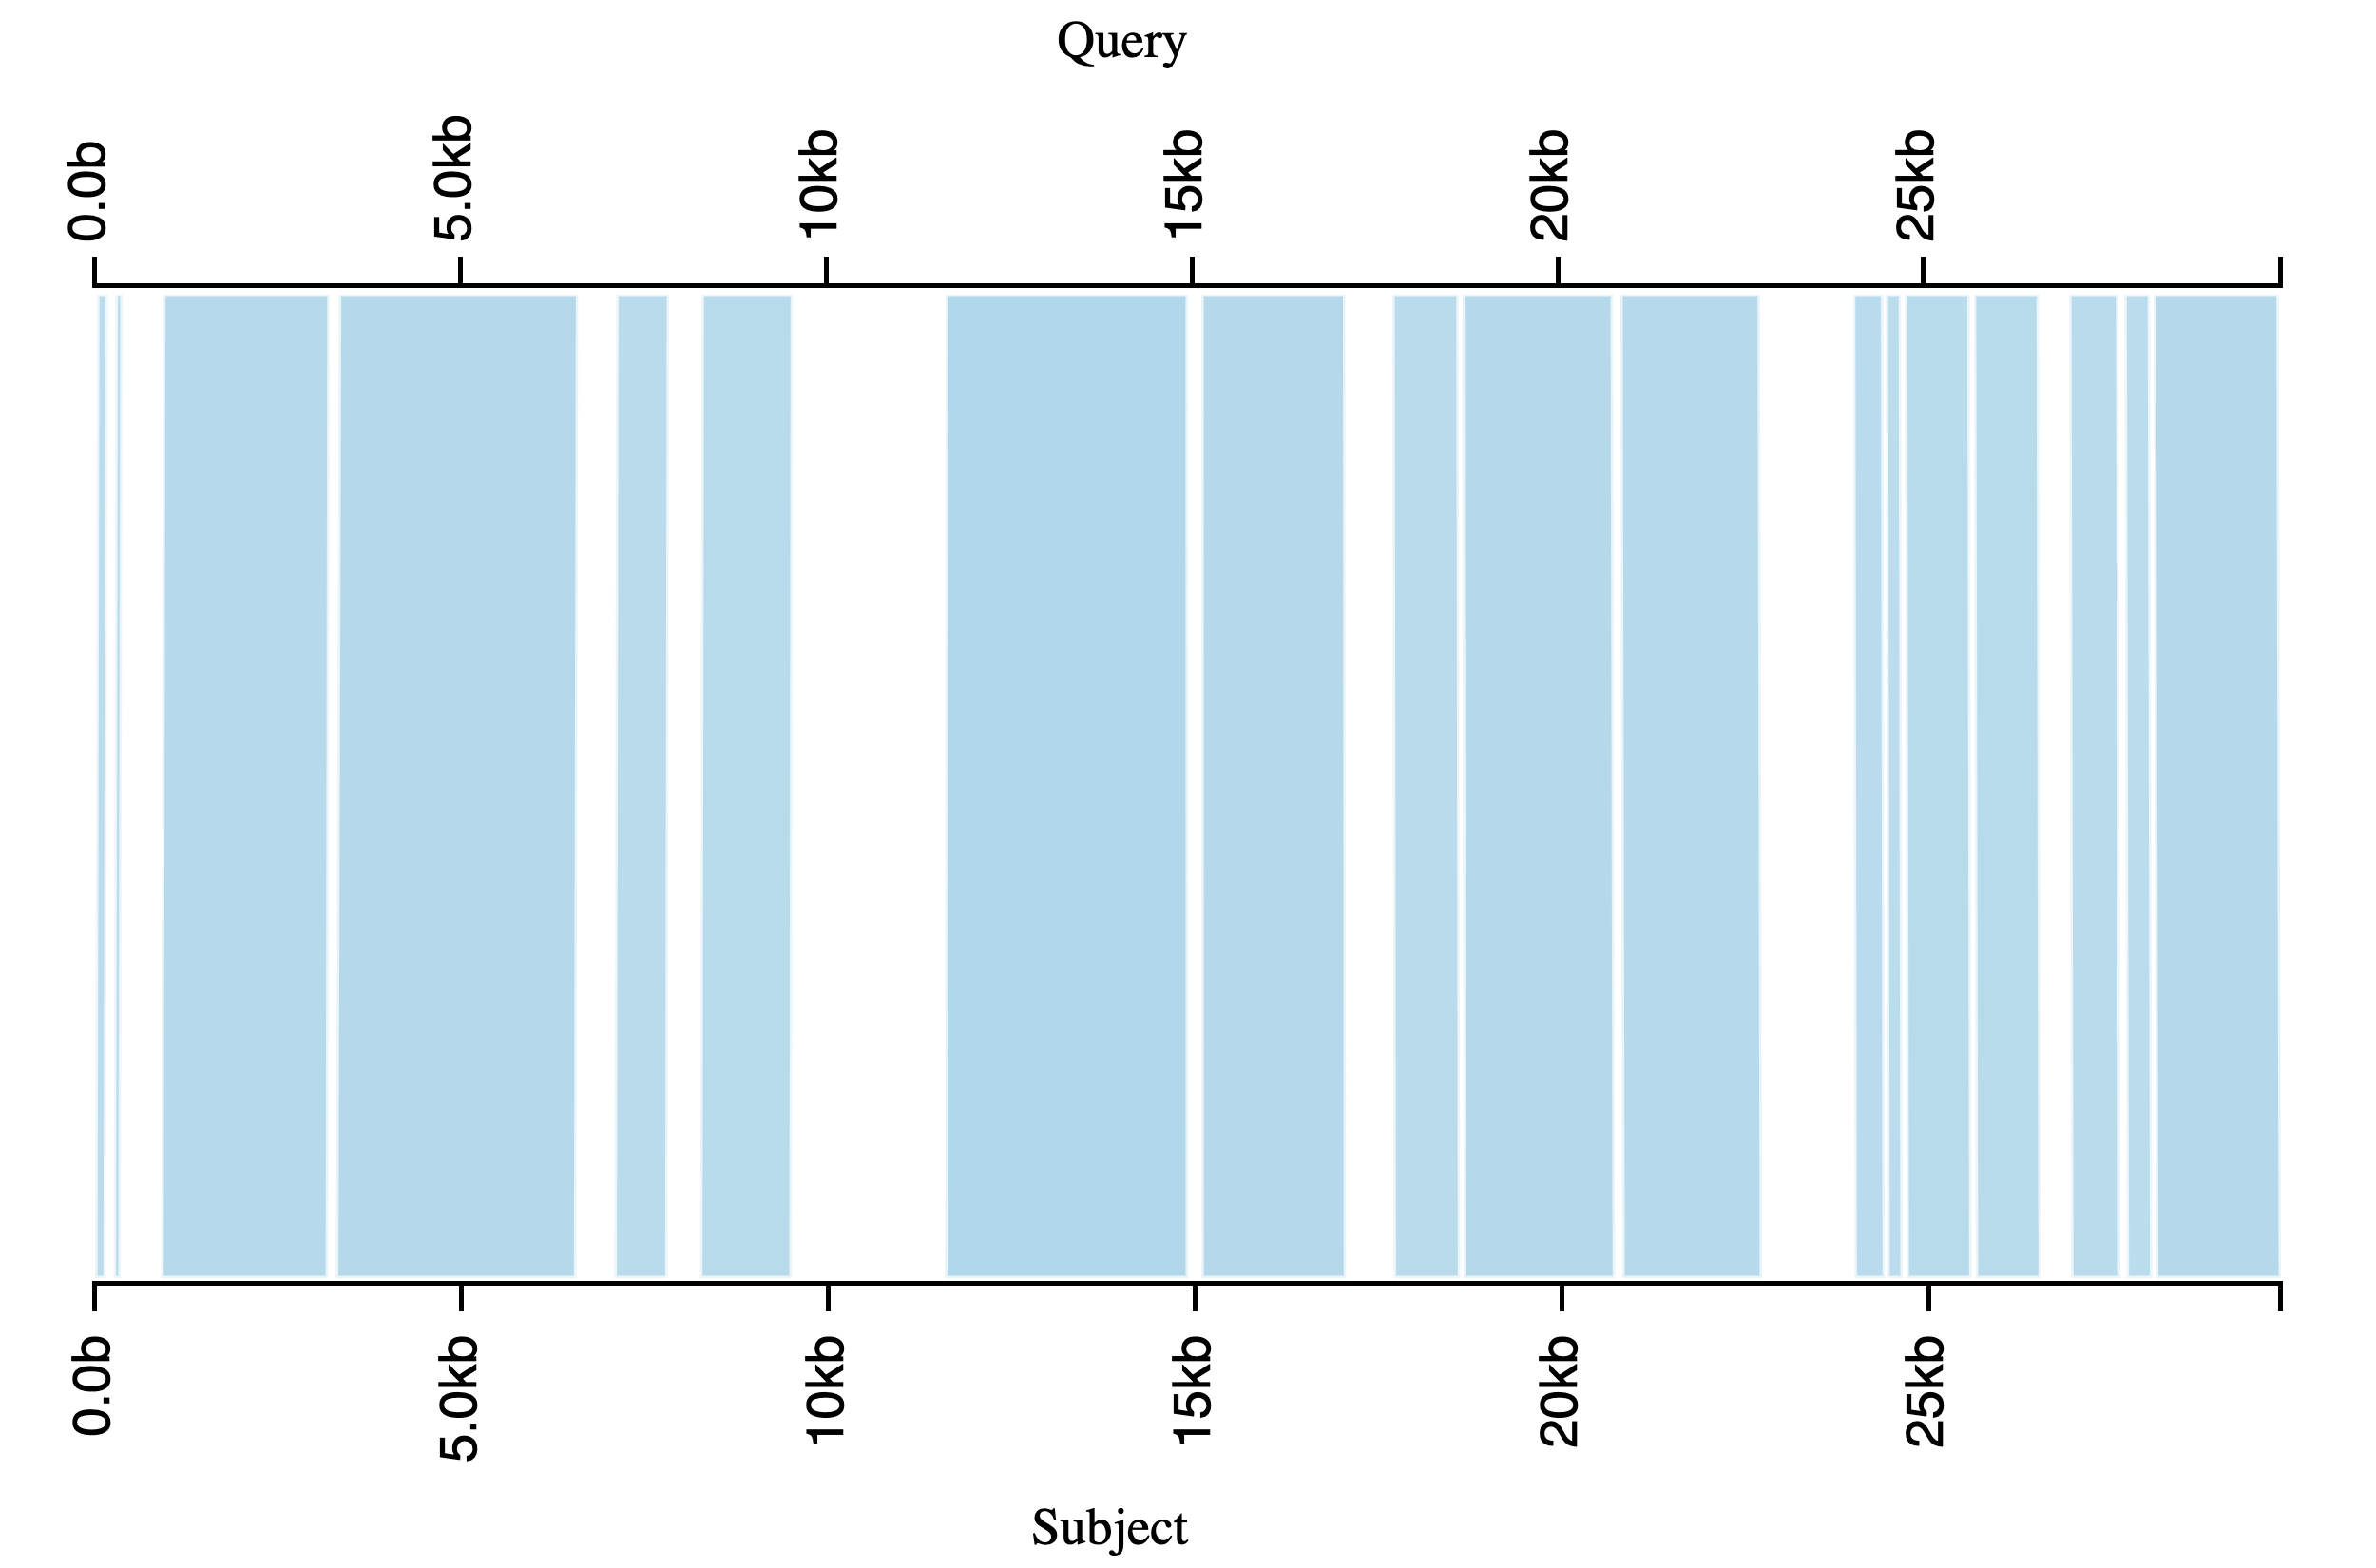
\includegraphics[width=1.8in]{B5}}
  \subfigure[BetaCoV\_pangolin\_Guangxi\_P2S]{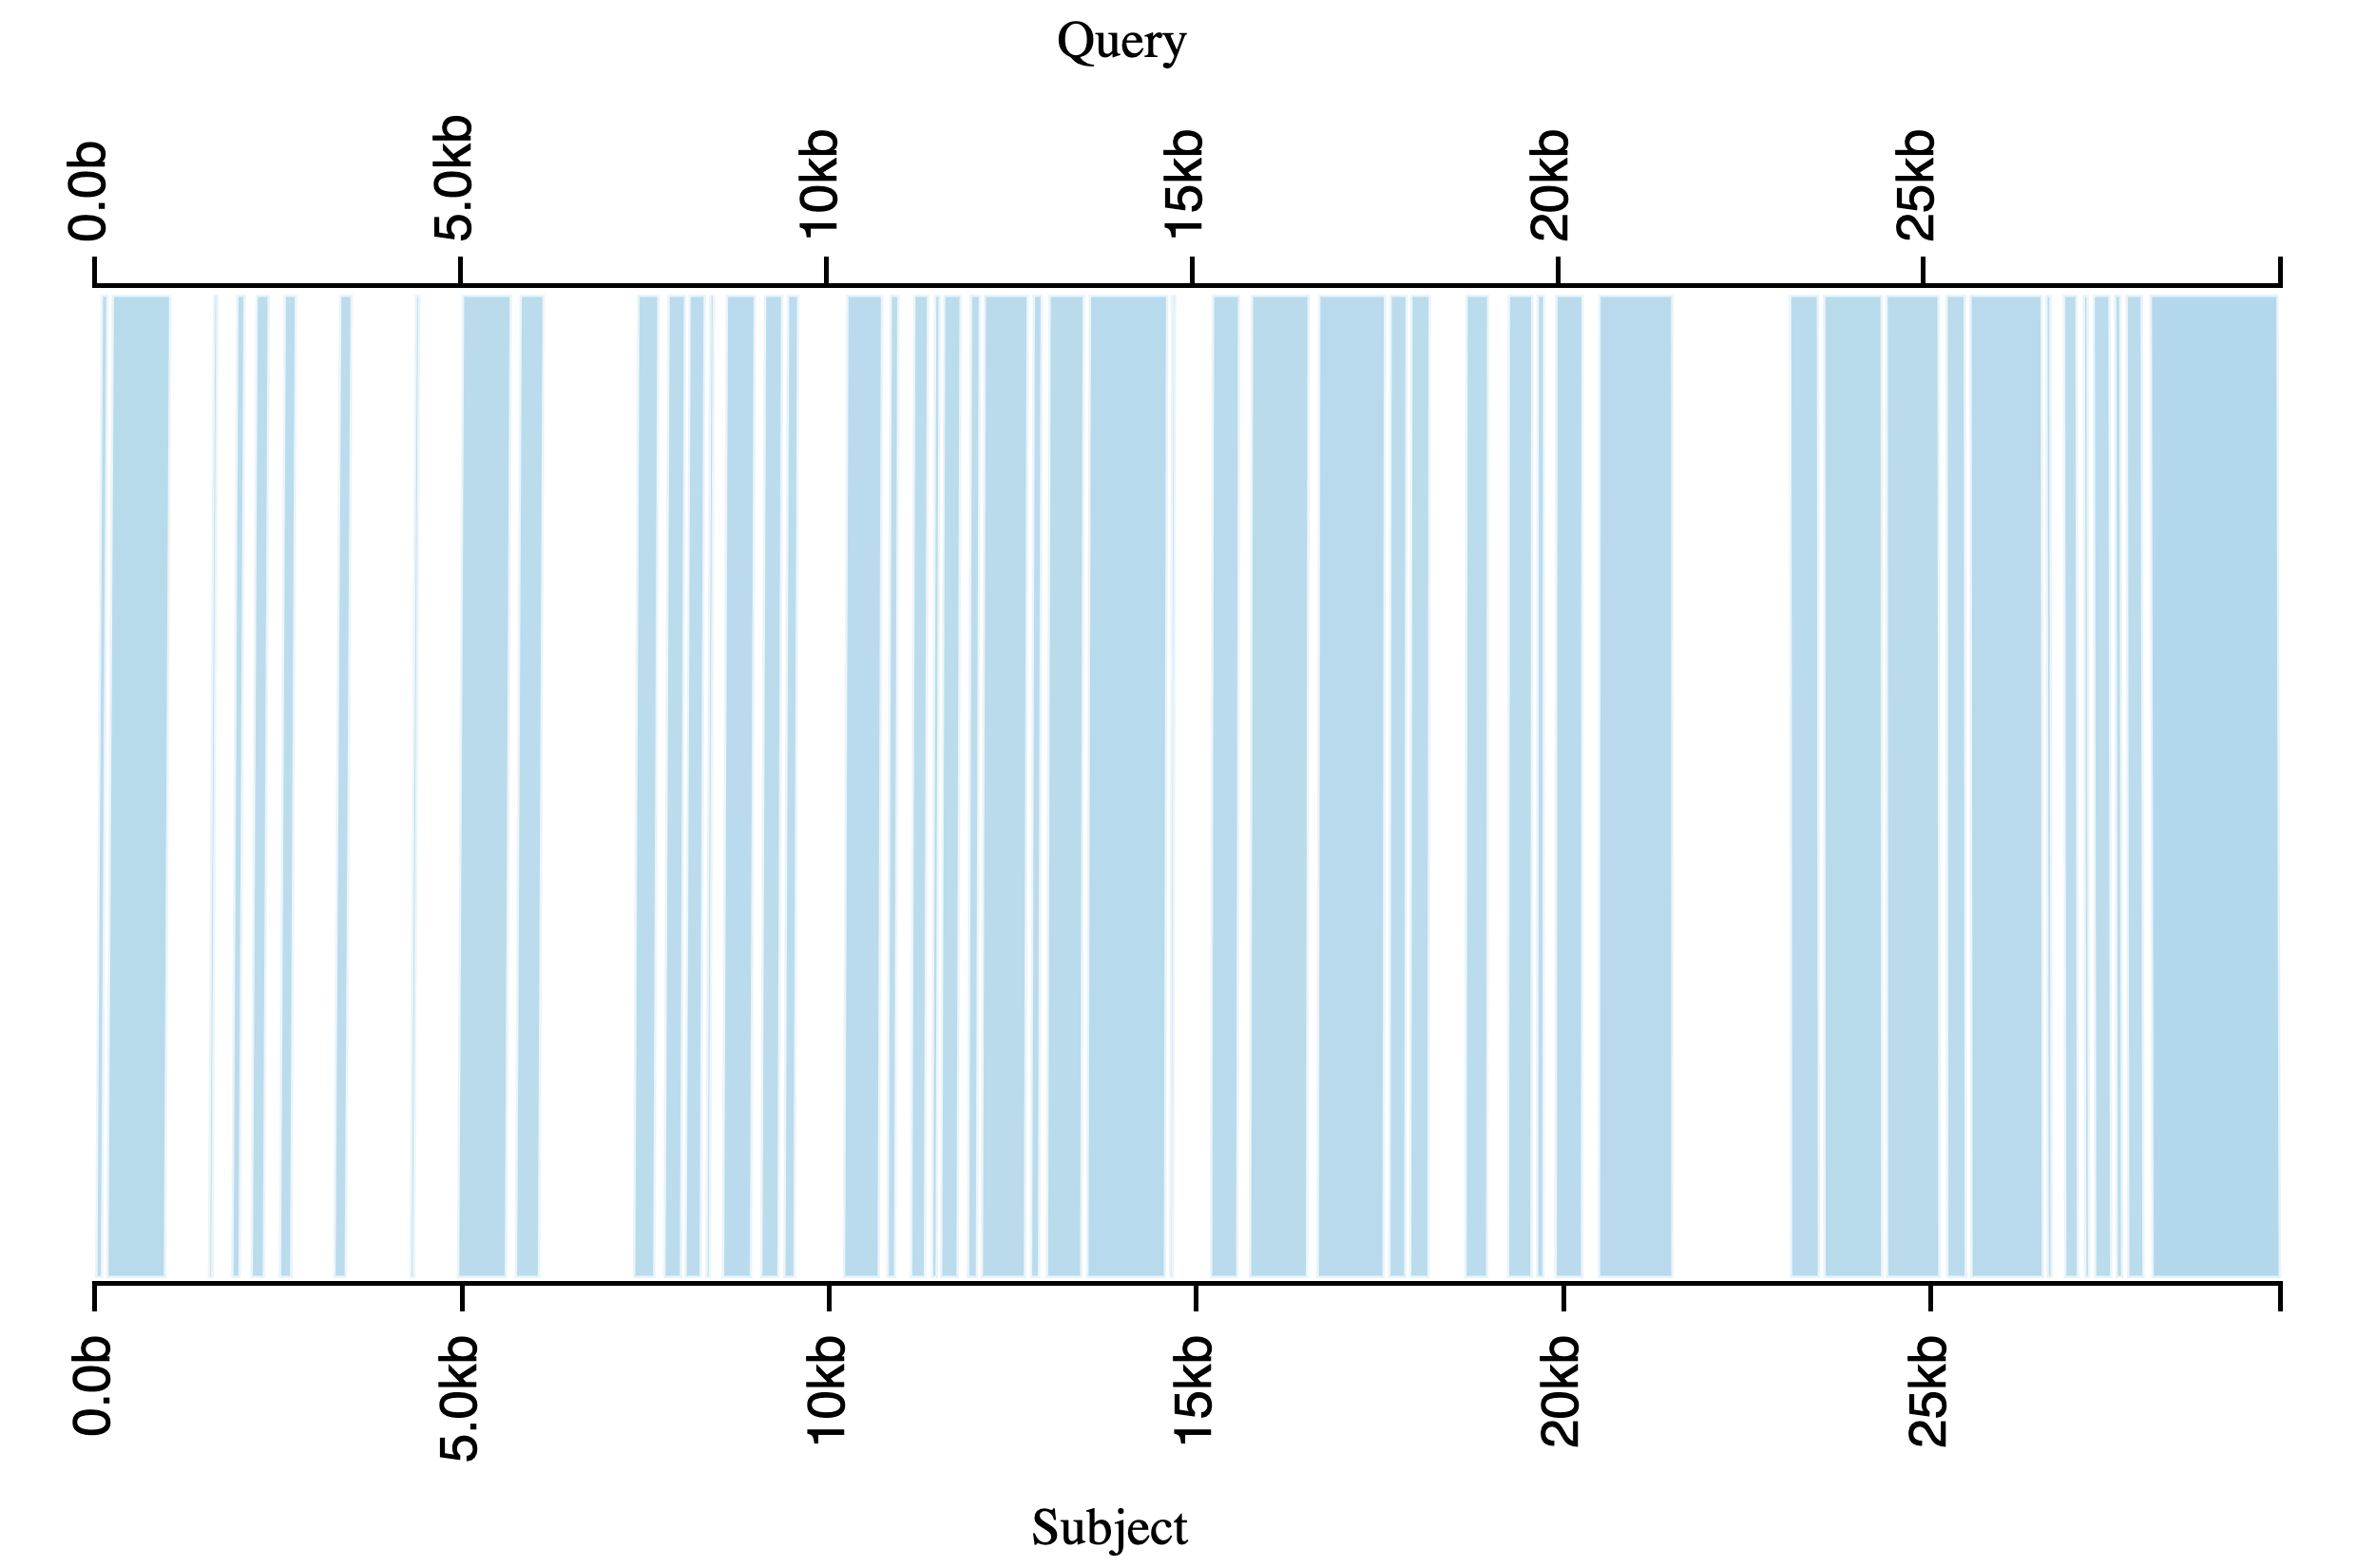
\includegraphics[width=1.8in]{B6}}
  \caption{Typical results of Blasting MT186683\upcite{wintersinger2015kablammo}}
  \label{fig1} %% label for entire figure
\end{figure}

\subsubsection{Preprocessing the query}
First, we took a overview of the query file:
\begin{lstlisting}
root@2cfa8ee205ce:~/exp5# head query1.fasta 
>MT186683.1 Severe acute respiratory syndrome coronavirus 2 isolate SARS-CoV-2/human/HKG/HK20/2020, complete genome
ATTAAAGGTTTATACCTTCCCAGGTAACAAACCAACCAACTTTCGATCTCTTGTAGATCTGTTCTCTAAA
CGAACTTTAAAATCTGTGTGGCTGTCACTCGGCTGCATGCTTAGTGCACTCACGCAGTATAATTAATAAC
...
\end{lstlisting}
As is shown above, the query file is a well-formatted nucleotide fasta file,
which is compatible with the \lstinline{blastn} tool.\upcite{zhang2000greedy} 

\subsubsection{Blasting the query with default parameters}
We used the default parameters to blast the query sequence.

\begin{lstlisting}
root@2cfa8ee205ce:~/exp5# time blastn -query query1.fasta -out out1.blast -db db

real	0m3.898s
user	0m0.793s
sys	0m0.078s
root@2cfa8ee205ce:~/exp5# head -n 30 out1.blast 
BLASTN 2.11.0+


Reference: Zheng Zhang, Scott Schwartz, Lukas Wagner, and Webb
Miller (2000), "A greedy algorithm for aligning DNA sequences", J
Comput Biol 2000; 7(1-2):203-14.



Database: db.fasta
           198 sequences; 5,904,042 total letters



Query= MT186683.1 Severe acute respiratory syndrome coronavirus 2 isolate
SARS-CoV-2/human/HKG/HK20/2020, complete genome

Length=29888
                                                                      Score     E
Sequences producing significant alignments:                          (Bits)  Value

MN908947 |Severe acute respiratory syndrome coronavirus 2 isolate...  55177   0.0  
MN996528 |Severe acute respiratory syndrome coronavirus 2 isolate...  55177   0.0  
MT019532 |Severe acute respiratory syndrome coronavirus 2 isolate...  55177   0.0  
NC_045512 |Severe acute respiratory syndrome coronavirus 2 isolat...  55177   0.0  
BetaCoV/Wuhan/WIV04/2019|EPI_ISL_402124                               55177   0.0  
NC_045512.2 Wuhan seafood market pneumonia virus isolate Wuhan-Hu...  55177   0.0  
MT019531 |Severe acute respiratory syndrome coronavirus 2 isolate...  55171   0.0  
MT192772 |Severe acute respiratory syndrome coronavirus 2 isolate...  55171   0.0  
MN994468 |Severe acute respiratory syndrome coronavirus 2 isolate...  55167   0.0  
\end{lstlisting}
Several significant results are produced by the program, with good Scores and E values.

\subsubsection{Blasting the best match of the query}
To show the best match, add some restrictions (\lstinline{-num_descriptions 1}) to the command:

\begin{lstlisting}
root@2cfa8ee205ce:~/exp5# time blastn -query query1.fasta -out out1.blast -db db -evalue 1e-5 -num_descriptions 1

real	0m2.538s
user	0m0.812s
sys	0m0.064s
root@2cfa8ee205ce:~/exp5# head -n 30 out1.blast 
BLASTN 2.11.0+


Reference: Zheng Zhang, Scott Schwartz, Lukas Wagner, and Webb
Miller (2000), "A greedy algorithm for aligning DNA sequences", J
Comput Biol 2000; 7(1-2):203-14.



Database: db.fasta
           198 sequences; 5,904,042 total letters



Query= MT186683.1 Severe acute respiratory syndrome coronavirus 2 isolate
SARS-CoV-2/human/HKG/HK20/2020, complete genome

Length=29888
                                                                      Score     E
Sequences producing significant alignments:                          (Bits)  Value

MN908947 |Severe acute respiratory syndrome coronavirus 2 isolate...  55177   0.0  


>MN908947 |Severe acute respiratory syndrome coronavirus 2 isolate 
Wuhan-Hu-1| complete genome
Length=29903

 Score = 55177 bits (29879),  Expect = 0.0
 Identities = 29885/29888 (99%), Gaps = 0/29888 (0%)
\end{lstlisting}
As is shown in the result, the best match has the Identity of 99\%, with E value = 0,
which indicates that the match is good enough in sequence similarity (high identity), 
and it is almost impossible to get this result with an unrelevant sequence by chance (E value very close to 0).

\subsubsection{Comments of the Blast results}
Considering the biological meaning behind the query and the result,
it is reasonable that \lstinline{SARS-CoV-2/human/HKG/HK20/2020 complete genome} 
is a good match with \lstinline{SARS-CoV-2 Wuhan-Hu-1 complete genome},
since they are both \lstinline{SARS-CoV-2} samples collected from different 
sources and sequenced by different institutes.
The two sequences has only three different bases, which can be seen as minor mutations or errors in sequencing.

\subsection{Blasting \texttt{NP\_002200}}

\subsubsection{Result overview}

\begin{figure}[H]
    \centering
    
\includegraphics[width=1\textwidth]{N1}
    \caption{AY572034.1, Alignments produced by TBLASTN, with E value = 74\upcite{wintersinger2015kablammo}}
    \label{N1}
\end{figure}

\subsubsection{Preprocessing the query}
First, we took a overview of the query file:
\begin{lstlisting}
root@2cfa8ee205ce:~/exp5# head query2.fasta 
>NP_002200.2 integrin alpha-L isoform a precursor [Homo sapiens]
MKDSCITVMAMALLSGFFFFAPASSYNLDVRGARSFSPPRAGRHFGYRVLQVGNGVIVGAPGEGNSTGSL
YQCQSGTGHCLPVTLRGSNYTSKYLGMTLATDPTDGSILACDPGLSRTCDQNTYLSGLCYLFRQNLQGPM
...
\end{lstlisting}
As is shown above, the query file is a well-formatted protein fasta file,
which is compatible with the \lstinline{tblastn} tool. 

\subsubsection{Blasting the query with default parameters}
We used the default parameters to blast the query sequence.

\begin{lstlisting}
root@2cfa8ee205ce:~/exp5# time tblastn -query query2.fasta -out out2.blast -db db

real	0m1.427s
user	0m0.193s
sys	0m0.003s                               
root@2cfa8ee205ce:~/exp5# cat out2.blast 
TBLASTN 2.11.0+


Reference: Stephen F. Altschul, Thomas L. Madden, Alejandro A.
Schaffer, Jinghui Zhang, Zheng Zhang, Webb Miller, and David J.
Lipman (1997), "Gapped BLAST and PSI-BLAST: a new generation of
protein database search programs", Nucleic Acids Res. 25:3389-3402.



Database: db.fasta
           198 sequences; 5,904,042 total letters



Query= NP_002200.2 integrin alpha-L isoform a precursor [Homo sapiens]

Length=1170


***** No hits found *****



Lambda      K        H        a         alpha
   0.319    0.137    0.409    0.792     4.96 

Gapped
Lambda      K        H        a         alpha    sigma
   0.267   0.0410    0.140     1.90     42.6     43.6 

Effective search space used: 2086749252


  Database: db.fasta
    Posted date:  Apr 23, 2021  3:05 PM
  Number of letters in database: 5,904,042
  Number of sequences in database:  198



Matrix: BLOSUM62
Gap Penalties: Existence: 11, Extension: 1
Neighboring words threshold: 13
Window for multiple hits: 40

\end{lstlisting}
As is shown above, the \lstinline{tblastn}\upcite{altschul_gapped_1997} tool did not give out a
significant match between the query sequence and the database.


\subsubsection{Blasting the best match of the query}
To get some acceptable results, we added some parameters to make
\lstinline{tblastn} more sensitive but less accurate (\lstinline{-e_value 1000}) to the command:

\begin{lstlisting}
root@2cfa8ee205ce:~/exp5# time tblastn -query query2.fasta -out out2.blast -db db -evalue 1000 -num_descriptions 1

real	0m2.170s
user	0m1.036s
sys	0m0.007s
root@2cfa8ee205ce:~/exp5# cat out2.blast 
TBLASTN 2.11.0+


Reference: Stephen F. Altschul, Thomas L. Madden, Alejandro A.
Schaffer, Jinghui Zhang, Zheng Zhang, Webb Miller, and David J.
Lipman (1997), "Gapped BLAST and PSI-BLAST: a new generation of
protein database search programs", Nucleic Acids Res. 25:3389-3402.



Database: db.fasta
           198 sequences; 5,904,042 total letters



Query= NP_002200.2 integrin alpha-L isoform a precursor [Homo sapiens]

Length=1170
                                                                      Score     E
Sequences producing significant alignments:                          (Bits)  Value

AY572034.1 SARS coronavirus civet007, complete genome                 25.0    74   


>AY572034.1 SARS coronavirus civet007, complete genome
Length=29540

 Score = 25.0 bits (53),  Expect = 74, Method: Compositional matrix adjust.
 Identities = 11/32 (34%), Positives = 14/32 (44%), Gaps = 0/32 (0%)
 Frame = -3

Query  553   IFNGRHGGLSPQPSQRIEGTQVLSGIQWFGRS  584
             I + R    S  PS  +      SGI+WF  S
Sbjct  1989  IASTRRNDCSKIPSSMVTAALCKSGIEWFAAS  1894
...
\end{lstlisting}
As is shown in the result, the best match has the Identity of 34\%, with E value = 74,
which indicates that the match is no better than random matches since it has a low similarity
and a high E value. As a rule of thumb, any results whose E value is larger than 1e-5 is
not desirable. If we consider the size of our database, E value = 74 means that one might expect to see 74 match with a similar score simply by chance,
which is almost non sense.

\subsubsection{Comments of the Blast results}
This result is not surprising since we are blasting human integrin sequence with a database
of sequences from \lstinline{SARS-CoV-2}, which has different origin than human. 
If the \lstinline{tblastn} gives out significant
results, it could be instersting to investigate in depth of the relationship between
human integrin and SARS-CoV-2.


\subsection{Benchmarking the tools}

The queries we made took less than 5 seconds to process, 
since the database we made is small enough.
We are curious how the time blast takes when we have a larger database, and
how the query length will affect the query time.
To carry out the benchmark, we chose the Swiss-Prot as the source to build 
our databases, and time different queries.

Below are the benchmark results.

\begin{figure}[H]
    \centering
    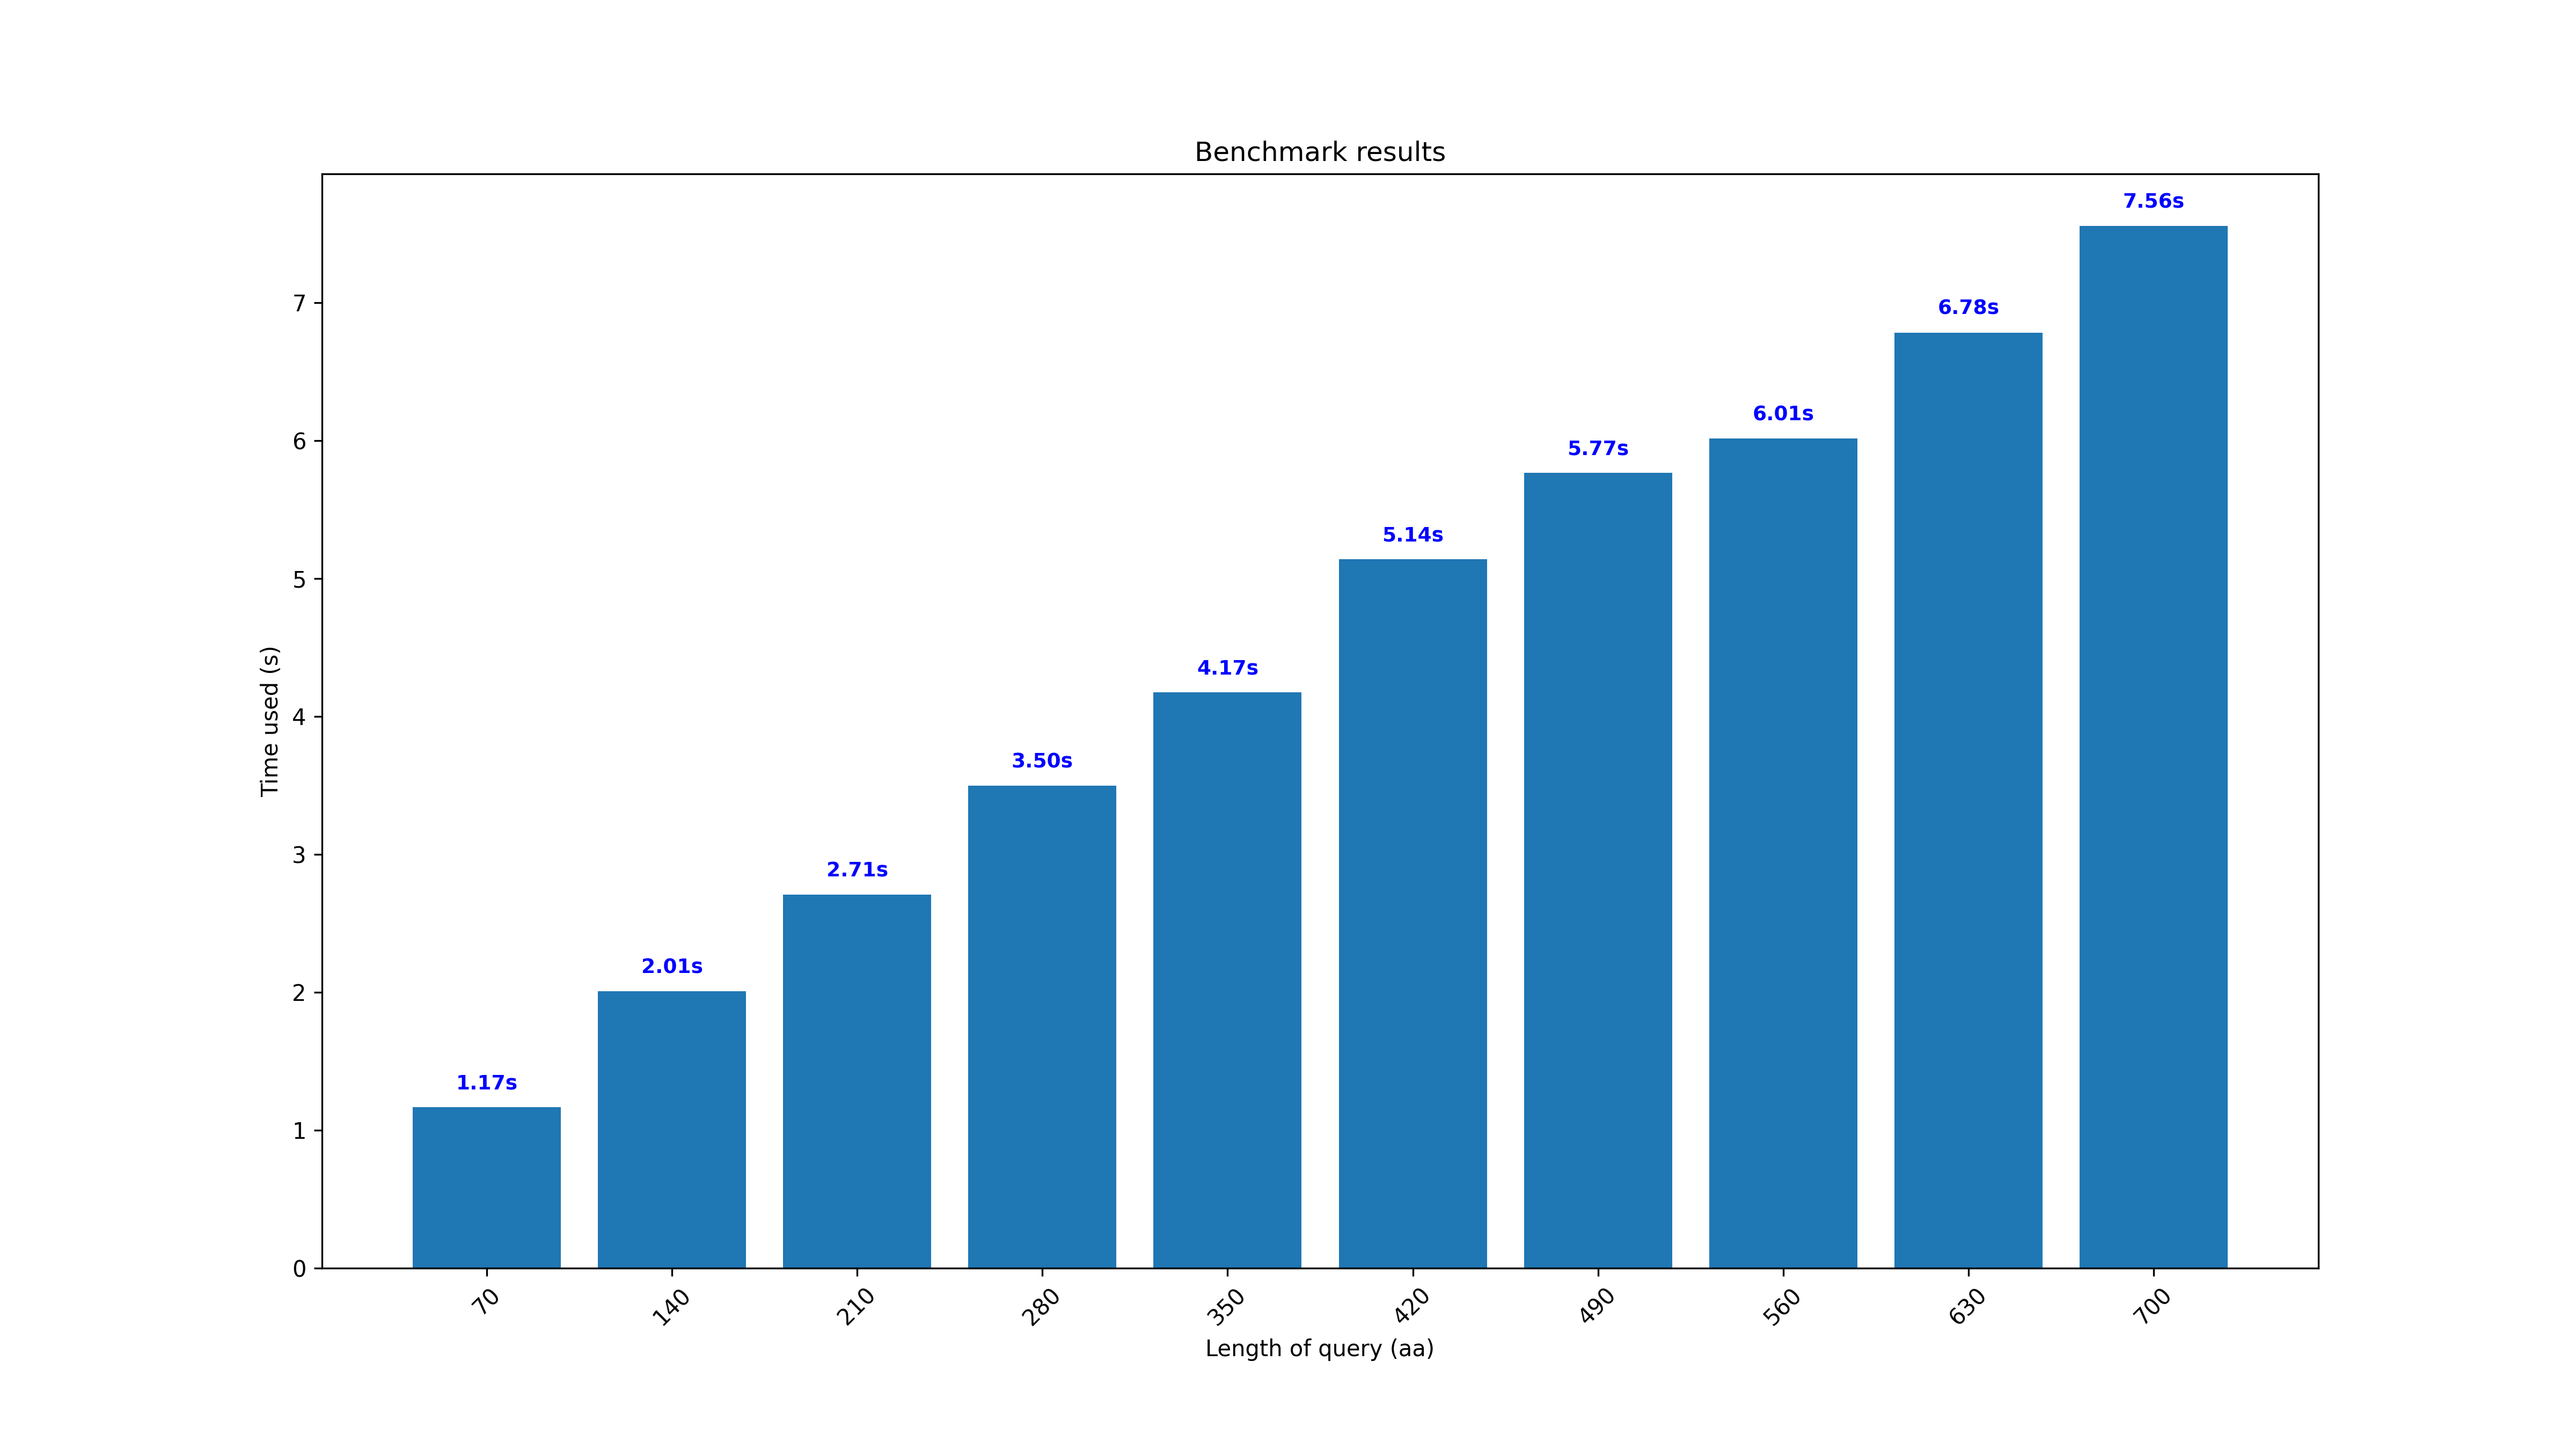
\includegraphics[width=1\textwidth]{Fig01}
    \caption{Benchmarking BLASTP with data from Swiss-Prot\upcite{boeckmann2003swiss}}
    \label{fig01}
\end{figure}

\section{Discussions}

From the blast results above,
we learnt how to build a customized blast database
and how to query a certain sequence in the database.
If the sequence we want to query is not compatible with
the database (eg. protein to nucleotide), the choice of the right
tool is necessary (blastn, blastp, blastx, tblastn, tblastx).
To choose the right tool, we can add \lstinline{-help} to the
commands to veiw the manual of the command.

The results given by blast can be adjusted by changing the
parameters, and therefore, when doing blast, reading papers or 
reporting your own results, take note of the parameters used.
Manipulation of the parameters can be useful to get
our desired results, but keep in mind that falsification or 
other kind of academic misconduct is forbidden.

Blast tools is believed to have the O(n) speed,
which seems to be true according to the breif benchmark.




\section{Supplementary materials}



\subsection{Environment of this experiment}
The hardware we used is a x86\_64 compatible machine,
and the software used in the experiment is shown in the table below.

\begin{table}[H]
    \caption{Software used in the experiment}
    \centering
    \begin{tabular}{cc}
        \toprule
        Name&Version\\
        \midrule
        OS: Ubuntu&18.04\\
        CXX Complier GCC&7.5.0\\
        BLAST&2.11.0+\\
        Curl&7.58.0\\
        \bottomrule
    \end{tabular}
\end{table}

\subsection{Fetch data from NCBI}
\begin{lstlisting}
# curl "https://eutils.ncbi.nlm.nih.gov/entrez/eutils/efetch.fcgi?db=nuccore&id=MT186683.1&rettype=fasta&retmode=text" > query1.fasta 
  % Total    % Received % Xferd  Average Speed   Time    Time     Time  Current
                                 Dload  Upload   Total   Spent    Left  Speed
100 30432    0 30432    0     0   3559      0 --:--:--  0:00:08 --:--:--  7060


# curl "https://eutils.ncbi.nlm.nih.gov/entrez/eutils/efetch.fcgi?db=protein&id=NP_002200.2&rettype=fasta&retmode=text" > query2.fasta 
  % Total    % Received % Xferd  Average Speed   Time    Time     Time  Current
                                 Dload  Upload   Total   Spent    Left  Speed
100  1253    0  1253    0     0    608      0 --:--:--  0:00:02 --:--:--   608
\end{lstlisting}


\bibstyle{unsrt}
\bibliography{references}{}
\end{document}
